\documentclass{article}

\usepackage{graphicx}
\usepackage{amsmath}
\usepackage[margin=1.5in]{geometry}
\usepackage{setspace}
\usepackage{indentfirst}
\usepackage{changepage}
\usepackage{titlesec}
\usepackage{float}
\usepackage{caption}
\usepackage{subcaption}

\onehalfspacing
\setlength\parindent{1cm}

\renewcommand{\figurename}{Gambar}
\renewcommand{\tablename}{Tabel}

\titleformat{\section}[block]{\bfseries}{\thesection.}{1em}{}
\titleformat{\subsection}[block]{\bfseries}{\thesubsection}{1em}{}
\titleformat{\subsubsection}[block]{\bfseries}{\thesubsubsection}{1em}{}
\titlespacing*{\subsection} {2em}{3.25ex plus 1ex minus .2ex}{1.5ex plus .2ex}
\titlespacing*{\subsubsection} {4em}{3.25ex plus 1ex minus .2ex}{1.5ex plus .2ex}

\begin{document}

\begin{titlepage}

\begin{center}
	
\textbf{Data Mining}

\vspace{0.5cm}
\textbf{GEMASTIK 8}

\vspace{1.5cm}

\textbf{Analisa Profit Divergence pada Data Pemesanan Taksi\\ Menggunakan Metode Kulback Leibler Divergence\\dengan Isotonic Regression dan K-Means Clustering}

\vspace{1.5cm}
\textbf{Disusun oleh:}\\
Joshua Casey Darian Gunawan\\
Muhammad Zaky Khairuddin\\
Zamil Majdy
\vspace{1.5cm}

\vspace{0.8cm}
ZJZ\\
FAKULTAS ILMU KOMPUTER\\
UNIVERSITAS INDONESIA\\
2015
\end{center}
\end{titlepage}

\tableofcontents
\newpage

\section{Latar Belakang}

Informasi adalah hal yang sangat penting. Informasi memungkinkan seseorang untuk bertindak dengan lebih relevan dengan keadaan saat itu. Dengan adanya informasi, keputusan dapat diambil dengan lebih tepat sehingga memperoleh hasil yang lebih optimal. Salah satu contoh pentingnya informasi adalah dalam bidang bisnis. Agar dapat menguasai dunia bisnis, kita harus mengetahui dan menguasai fenomena-fenomena yang terjadi di pasar. Dengan memiliki data tentang hal-hal yang terjadi di pasar, mengolahnya, dan mengambil informasi yang terdapat dalam data itu, kita dapat mengetahui kejadian di pasar, memprediksi apa yang mungkin terjadi, mengetahui keberadaan anomali dalam bisnis, serta mengambil langkah yang tepat.

Dewasa ini, bentuk konkrit dari informasi yang beredar adalah data. Data beredar dalam jumlah yang sangat banyak sehingga tidak mungkin dapat dilakukan pemprosesan data tersebut satu persatu. Padahal, informasi yang terkandung dalam data tersebut bisa jadi sangatlah bermanfaat. Oleh karena itu, diperlukan metode khusus untuk mengolah data sehingga informasi-informasi yang bermanfaat tersebut dapat diperoleh.

Dalam studi ilmu komputer, terdapat bidang yang khusus mempelajari pengolahan data dalam jumlah besar, yakni data mining. Teknik-teknik dalam data mining memungkinkan pengolahan data besar secara optimal sehingga informasi-informasi yang bermanfaat dapat diperoleh dari data tersebut. Salah satu contoh aplikasi data mining yang akan kami bahas dalam makalah ini adalah pengolahan terhadap dataset pemesanan taksi di daerah Portugal pada tanggal 1 Juli 2013 hingga 30 Juni 2014.


\section{Tujuan dan Manfaat}

Analisa yang kami lakukan bertujuan mencari dan menganlisa fenomena dan anomali keuntungan pasar pada penggunaan layanan taksi dengan pembagian berdasarkan daerah. Anomali yang dicari adalah anomali divergensi keuntungan, yakni perbedaan drastis keuntungan pada suatu daerah dengan skala waktu per bulan. Perbedaan drastis ini dapat berupa penurunan maupun kenaikan yang drastis. Keuntungan per daerah ini dihitung dengan memperhitungkan perjalanan-perjalanan dengan daerah tersebut sebagai titik awal maupun titik tujuan perjalanan.

Manfaat yang dapat diperoleh dari analisa ini adalah identifikasi daerah yang memiliki tingkat permintaan yang berubah drastis. Dengan mengetahui daerah-daerah yang mengalami perubahan tingkat permintaan yang tinggi, dapat dilakukan analisa bisnis yang memadai untuk memaksimalkan keuntungan, misalnya menambah armada di sekitar daerah yang permintaannya menaik drastis. Analisa ini akan sangat berguna apabila dilakukan stream data baru secara terus menerus perbulannya, agar hasil analisa ini dapat digunakan untuk mengambil kebijakan bisnis secara lebih real time.  Analisa dari segi bisnis secara khusus tidak dibahas dalam makalah ini.

\section{Batasan}

Pada penelitian ini penulis melakukan pengamatan terhadap data yang memiliki daytype A, yakni hari kerja. Hal ini dilakukan karena daytype A paling umum ditemui diantara ketiga daytype tersebut, sementara setiap daytype tentu memiliki distribusi dan karakteristik yang sangat berbeda, sehingga tidak mungkin melakukan evaluasi yang sama terhadap ketiga daytype tersebut. Karena data yang harus diproses relatif banyak, algoritma yang digunakan adalah algoritma-algoritma yang memiliki kompleksitas rendah, misalnya k-means clustering algorithm dan  isotonic regression yang memiliki kompleksitas linear terhadap banyaknya data.

\section{Metode}

\subsection{Perangkat Lunak}

\subsubsection{WEKA Visualization and Learning Library}
\begin{adjustwidth}{4em}{0pt}

\hspace{\parindent}WEKA adalah \textit{learning} dan \textit{visualization} \textit{library} yang di kembangkan menggunakan bahasa Java. \textit{Library} ini memiliki banyak implementasi pemrosesan data dan algoritma learning yang cukup beragam seperti Support Vector Machine, Artificial Neural Network, dan tentu algoritma utama yang di pakai pada project ini yaitu K-Means dan Isotonic Regression (algoritma ini ada pada Weka Additional Package). Kelebihan library Java dibandingkan library lain adalah nature bahasa Java yang bisa di optimasi dan cukup cepat dibandingkan \textit{library} lain (dalam kasus ini adalah library python \footnote{http://benchmarksgame.alioth.debian.org/u64q/python.html}). Metode analisa pada kasus  ini membutuhkan data secara utuh (tidak melalui metode sampling) sehingga pemrosesan data dengan cepat sangat dibutuhkan pada kasus ini. Sehingga library ini merupakan pilihan yang cukup tepat.

\end{adjustwidth}

\subsubsection{ChartJS}
\begin{adjustwidth}{4em}{0pt}
	
\hspace{\parindent}Chart JS merupakan library dengan bahasa Javascript yang digunakan untuk melakukan visualisasi data dalam bentuk chart. Chart JS ini dipilih karena library ini merupakan library yang cukup ekstensif dan dapat digunakan untuk berbagai pemodelan data.

\end{adjustwidth}

\subsubsection{Google Fusion Tables}
\begin{adjustwidth}{4em}{0pt}
	
\hspace{\parindent}Google Fusion Tables adalah sebuah aplikasi web untuk visualisasi dan sharing data. Google Fusion Tables dapat membuat visualisasi berbentuk peta dengan bantuan Google Maps. Aplikasi ini digunakan dalam pembuatan heatmap. Keunggulan dari aplikasi ini adalah visualisasi yang dihasilkan cukup jelas dan sesuai dengan kebutuhan pengolahan data.

\end{adjustwidth}
\subsubsection{Python (Scikit-Learn \& GGplot)}
\begin{adjustwidth}{4em}{0pt}
		
\hspace{\parindent}Python pada kasus ini digunakan untuk melakukan prototyping, untuk mengevaluasi data sample yang berjumlah kecil untuk menguji model algoritma yang diberikan pada data. Python dipilih karena kemudahan implementasinya dan dapat kembangkan dengan cepat. Semua algoritma yang dikembangkan disini diimplementasikan ulang menggunakan Java untuk data utuh.

\end{adjustwidth}

\subsection{Dataset}

\begin{adjustwidth}{2em}{0pt}

\hspace{\parindent}Dataset yang digunakan adalah data taxi service trip yang merupakan data penggunaan jasa taxi yang tercatat pada (hari Senin 01 Juli 2013 00:00:58 GMT sampai dengan Senin, 30 Juni 2014 19:39:07 GMT). Terdapat 1710670 penggunaan jasa taxi pada interval waktu tersebut, hanya 10 penggunaan yg tidak memiliki keterangan data yang lengkap.

Dataset memiliki 9 atribut, yaitu \textit{trip\_id}, \textit{call\_type}, \textit{origin\_call}, \textit{origin\_stand}, \textit{taxi\_id}, \textit{timestamp}, \textit{day\_type}, \textit{missing}, dan \textit{polyline}. Penjelasan untuk masing-masing atribut adalah sebagai berikut:

\begin{itemize}
\item{\textit{trip\_id} : ID untuk setiap trip penggunaan taxi}
\item{\textit{call\_type} : Tipe penggunaan jasa taxi (A : permintaan langsung ke pusat, B : permintaan langsung ke supir taxi, C : penggunaan jasa taxi di tengah jalan)}
\item{\textit{origin\_call} : ID nomor telepon pemesan (hanya untuk call\_type A)}
\item{\textit{origin\_stand} : ID stand taxi (hanya untuk call\_type B)}
\item{\textit{taxi\_id} : ID supir taxi}
\item{\textit{timestamp} : Unix Timestamp (dalam detik). yg menandakan waktu mulai perjalanan.}
\item{\textit{day\_type} :  Tipe hari pemesanan (A : hari kerja, B : hari libur, C : hari sebelum hari libur)}
\item{\textit{missing} : Boolean (False jika data gps utuh, True jika data gps ada yang hilang)}
\item{\textit{polyline} : Data koordinat gps (WGS84 format) perjalanan taxi selama 15 detik}
\end{itemize}

\end{adjustwidth}

\subsection{Algoritma dan Teknik}

\subsubsection{K-Means}
\begin{adjustwidth}{4em}{0pt}

\hspace{\parindent}K-means adalah salah satu metode clustering yang populer digunakan dalam penerapan data mining. K-means dibangun dari ide bahwa 2 buah data yang memiliki kemiripan akan dikelompokkan ke dalam sebuah cluster. Kemiripan diukur dari jarak Euclidean (Euclidean distance) dari 2 buah data. Dalam kasus ini, jarak Euclidean dihitung dengan cara jarak Euclidean antara centroid data perjalanan yang tercatat oleh \textit{gps} pada data.

Euclidean distance antara titik a dan b dihitung sebagai berikut:
\begin{align*}
	dist(a,b) &= \sqrt{(x_{a} - x_{b})^2 + (y_{a} - y_{b})^2}
\end{align*}

Sebanyak k buah centroid (titik tengah) diambil secara acak. Kemudian dilakukan iterasi hingga konvergen. 

\end{adjustwidth}

\subsubsection{Davis Bouldin Index}

\begin{adjustwidth}{4em}{0pt}

\hspace{\parindent}Permasalahan terbesar dari \textit{k-means} adalah menentukan nilai k terbaik. Sulit untuk mengetahui berapa \textit{cluster} yang dapat terbentuk dari sebuah dataset. Untuk itu, penulis akan melakukan percobaan dengan beberapa buah nilai k dan menentukan mana yang terbaik dengan menghitung Davies Bouldin Index dari masing-masing \textit{cluster}.

\textit{Davies Bouldin Index} (DBI) adalah indeks pengukuran validitas model \textit{clustering} berdasarkan kemiripan dan perbedaan dari \textit{cluster-cluster}. Model \textit{clustering} dinilai semakin baik apabila anggota-anggota \textit{cluster}-nya saling berdekatan dan jarak antar \textit{cluster} semakin jauh. Nilai DBI yang lebih rendah menandakan model \textit{clustering} yang lebih baik.

DBI dihitung dengan cara:
\begin{align*}
DB_{k} &= \frac{1}{k}\sum\limits_{i=1}^k
\max\limits_{j=1,...,k,i\neq j}\frac{diam(c_i +) + diam(c_j)}{dist(z_i,z_j)}
\end{align*}

\begin{align*}
diam(c_i) &= \sqrt{\frac{1}{n_i}\sum\limits_{x\in c_i}dist(x,z_i)^2}
\end{align*}

\begin{itemize}
	\setlength{\itemindent}{1cm}
	\item{$c_i$ adalah cluster}
	\item{diam($c_i$) adalah diameter cluster $c_i$}
	\item{n adalah banyaknya titik}
	\item{$z_i$ adalah centroid cluster $c_i$}
	\item{dist(a,b) adalah \textit{euclidean distance} antara titik a dan b}
\end{itemize}

\end{adjustwidth}

\subsubsection{Haversine Formula}

\begin{adjustwidth}{4em}{0pt}
	
\hspace{\parindent}Haversine Formula adalah salah satu formula trigonometri yang digunakan untuk menghitung great circle distance, yakni jarak terdekat antara 2 titik pada permukaan bola dengan melalui permukaan bola tersebut. Haversine formula menghitung great circle distance dari 2 titik pada permukaan bola dengan parameter latitude dan longitude dari kedua titik tersebut.

Haversine formula didefinisikan sebagai berikut:
\begin{align*}
haversin(\frac{d}{r}) &= haversin(\phi _{2} - \phi _{1}) + cos(\phi _{1})cos(\phi _{2})haversin(\lambda _{2} - \lambda _{1})
\end{align*}
\begin{itemize}
	\setlength{\itemindent}{1cm}
	\item{d adalah \textit{great circle distance} antara tiitk 1 dan 2}
	\item{r adalah jari-jari bola}
	\item{$\phi$ adalah latitude}
	\item{$\lambda$ adalah longitude}
	\item{\textit{haversin} adalah fungsi trigonometri $haversin(\theta) = sin^2(\frac{\theta}{2}) = \frac{1-cos(\theta)}{2}$}
\end{itemize}

\end{adjustwidth}

\subsubsection{Isotonic Regression}
\begin{adjustwidth}{4em}{0pt}
	
\hspace{\parindent}Isotonic regression merupakan varian dari algoritma regresi yang memepertahankan arah trend dari perdictor regresi (fungsi regresi dipastikan monoton menaik atau menurun). Secara matematis definisi isotonic regression adalah sebagai berikut : diberikan data dengan nilai a1,a2,...,an, regresi F(x) merupakan fungsi monoton $(F(i) <= F(j) | i <= j)$  dengan nilai $\sum\limits_{i=1}^n({f(i)-a_{i}})^2$ seminimal mungkin.

Sifat monotonik ini dimanfaatkan untuk melakukan pendekatan  non-linear yang lebih akurat akan tetapi tidak membuat aproksimasinya menjadi overfit. Pada data yang bersangkutan, regresi ini digunakan untuk mengaproksimasi perkembangan divergensi profit pemesanan taxi.

\begin{figure}[H]
	\includegraphics[width=\linewidth]{isotonic.png}
	\caption{Contoh \textit{isotonic regression}}
\end{figure}

\end{adjustwidth}

\subsubsection{Kullback Leibler Divergence}
\begin{adjustwidth}{4em}{0pt}
\hspace{\parindent}Kullback Leibler Divergence merupakan salah satu teknik penghitungan divergensi dari distribusi dua nilai (pada umumnya distribusi probabilitas). Kullback Leibler Divergence pada distribusi data  P dan Q  didefinisikan sebagai 
$D_{Kl}(P||Q) = \sum\limits_{i}P(i)ln\frac{P(i)}{Q(i)}$
dengan P(i) merupakan nilai tendensi dari data ke-i pada dataset-P dan Q(i) merupakan nilai tendensi dari data ke-i pada dataset-Q.

Pada kasus ini, KL Divergence digunakan untuk menghitung divergensi dari dua nilai estimated score yaitu estimasi probabilitas (persentase) profit dari suatu daerah pada cluster tertentu. Estimated score ini  yang akan menjadi attribute utama untuk membandingkan divergensi profit yang akan dianalisis.

\end{adjustwidth}

\subsection{Teknik}

\begin{adjustwidth}{2em}{0pt}

\hspace{\parindent}Dalam penelitian ini, teknik-teknik yang digunakan antara lain:

\end{adjustwidth}

\subsubsection{Preprocessing}

\begin{adjustwidth}{4em}{0pt}

\hspace{\parindent}Sebelum dataset diproses, perlu dilakukan langkah-langkah tertentu terlebih dahulu agar dataset tersebut lebih mudah untuk diproses dan sesuai dengan kriteria yang diinginkan. Langkah-langkah yang diambil dalam preprocessing antara lain:

\begin{itemize}
	\item{Data Filtering}
		
		Data filtering adalah proses pembuangan data-data yang tidak memenuhi batasan yang ditentukan. Pembuangan data yang tidak memenuhi batasan dilakukan agar hasil penilitian relevan dengan batasan tersebut dan proses evaluasi dan analisa data menjadi lebih mudah dan cepat karena tidak ada data sampah yang terlibat dalam komputasi-komputasi yang dilakukan.
		
	\item{Data Standardization dan Meta Data Customization}
		
		Standarisasi data termasuk mengatur kembali banyaknya baris atau kolom pada dataset dan mengubah nilai yang ada menjadi kisaran tertentu, misalnya data nominal dijadikan numerik, boolean, atau lainnya. Dalam penelitian ini, penulis melakukan standarisasi data, yaitu mengubah nilai-nilai numerik menjadi nilai probabilitasnya (persentase).
		
	\item{Feature Extraction}
		
		Feature extraction adalah pengurangan atribut pada dataset apabila ukuran dataset terlalu besar atau ada atribut yang berulang (redundant). Dalam penelitian ini, kami mengabaikan atribut call type, origin call, origin stand, dan taxi id, karena tidak relevan dengan tujuan analisa yang dilakukan.
		
\end{itemize}

\end{adjustwidth}

\subsubsection{Modeling}
\begin{adjustwidth}{4em}{0pt}
	
\hspace{\parindent}Setelah melalui tahap preprocessing, data akan dimodelkan untuk menggambarkan distribusi data tersebut dan hubungan antara data yang satu dengan yang lain. Pada penelitian ini, teknik modeling yang digunakan antara lain: 

\begin{itemize}
	\item{Clustering}
	
	Clustering adalah teknik mengelompokkan data yang memiliki kemiripan karakteristik dan menjadikan data yang memiliki kesamaan karakteristik tersebut menjadi 1 kelompok.
	
	\item{Regression Line Fitting}
	
	Regression line fitting adalah teknik mengaproksimasi trend data dengan membentuk fungsi regresi yang mendekati distribusi data asli dan melakukan prediksi terhadap fluktuasi data dengan menggunakan fungsi regresi tersebut.
	
\end{itemize}

\end{adjustwidth}

\subsubsection{Inference}

\begin{adjustwidth}{4em}{0pt}
	
\hspace{\parindent}Inferensi (penarikan kesimpulan) dilakukan terhadap hasil modeling pada langkah sebelumnya dengan menerapkan perhitungan dan konsep matematis dengan pendekatan statistik sehingga diperoleh informasi yang berkaitan dengan tujuan pengolahan data yang telah dipaparkan pada bagian sebelumnya.

\end{adjustwidth}

\section{Desain dan Implementasi}

\subsection{Desain}

\begin{adjustwidth}{2em}{0pt}

\begin{figure}[H]
	\centering
	\includegraphics[width=0.8\linewidth]{Design.png}
	\caption{Rancangan pengolahan dataset}
\end{figure}

\hspace{\parindent}Langkah pertama yang dilakukan pada data adalah preprocessing sehingga data tersebut siap untuk melalui langkah-langkah berikutnya. Langkah kedua adalah melakukan clustering terhadap data tersebut. Langkah berikutnya yaitu membuat time series, yaitu data berisi pendapatan masing-masing cluster yang diurutkan berdasarkan waktu. Setelah itu, data tersebut akan dibaca dengan terbagi setiap bulannya. Data per bulan tersebut akan melalui sistem scoring kemudian divisualisasi.

\end{adjustwidth}

\subsection{Preprocessing}

\begin{adjustwidth}{2em}{0pt}

\begin{figure}[H]
	\centering
	\includegraphics[width=0.8\linewidth]{Preprocess.png}
	\caption{Teknik \textit{preprocessing} dataset}
\end{figure}

\hspace{\parindent}Sebelum diolah lebih lanjut, dataset yang diterima akan diproses terlebih dahulu. Langkah awal pemrosesan awal ini adalah membuang data yang tidak termasuk dalam batasan analisa ini. Setelah itu, kami melakukan pemisahan data. Tiap data kami pecah menjadi dua data, dengan data yang pertama memuat titik awal perjalanan dan data yang kedua memuat titik akhir perjalanan. Terakhir, atribut-atribut baru ditambahkan pada data.

\end{adjustwidth}

\subsubsection{Filter Unused Data}

\begin{adjustwidth}{4em}{0pt}
	
\hspace{\parindent}Sebelum memproses data lebih lanjut, langkah pertama yang dilakukan adalah membuang data yang tidak sesuai. Data yang kami buang adalah data yang memiliki stream gps yang tidak lengkap, karena membuat data secara keseluruhan tidak akurat, sementara jumlahnya yang sangat sedikit dibandingkan dengan keseluruhan data hampir tidak menimbulakan pengaruh ketika data dianulir. Selain itu, data yang kami buang adalah data yang tipe harinya bukan hari kerja, karena tidak sesuai untuk analisa dalam batasan yang telah ditentukan.

\end{adjustwidth}

\subsubsection{Feature Extraction}

\begin{adjustwidth}{4em}{0pt}
	
	\hspace{\parindent}Agar data lebih mudah diproses, atribut-atribut yang tidak sesuai dengan tujuan dari analisa ini dihilangkan dari dataset. Atribut-atribut tersebut antara lain daytype (karena hanya digunakan saat filtering), call type, origin stand, origin call, taxi id, dan trip id.
	
\end{adjustwidth}

\subsubsection{Split Data}

\begin{adjustwidth}{4em}{0pt}
	
	\hspace{\parindent}Masing-masing data yang telah difilter dipecah menjadi 2 data yang berbeda. Data x akan dipecah menjadi data x1 dan x2, dimana x1 memuat koordinat awal perjalanan dari x dan x2 memuat koordinat akhir perjalanan dari x. Hal ini dilakukan karena dalam batasan yang ditentukan, data yang diperlukan adalah traffic dari suatu daerah secara keseluruhan, baik dari maupun ke suatu daerah.
	
\end{adjustwidth}

\subsubsection{Add Attributes}

\begin{adjustwidth}{4em}{0pt}
	
	\hspace{\parindent}Setelah dilakukan pemecahan data, atribut baru yang diperlukan untuk komputasi ditambahkan ke dalam data tersebut. Atribut-atribut tersebut antara lain:
	
	\begin{itemize}
		\item{Total Distance}
		
		Total distance adalah jarak yang dilewati oleh taksi tersebut selama perjalanan. Total Distance dihitung dengan total  great circle distance antar titik pada gps stream. Masing-masing great circle distance tersebut dihitung dengan menggunakan formula Haversine.
		
		\item{Gross Profit Estimation}
		
		Gross Profit Estimation adalah esitimasi  total keuntungan  yang diperoleh sebuah layanan taksi pada perjalanan tersebut. Gross profit ini digunakan untuk mempermudah representasi data. Esitimasi ini dihitung menggunakan formula yang tidak mengubah proporsi rasio data pemesanan terhadap data lain yang diperoleh berdasarkan time-rate dan distance-rate. Formula yang digunakan adalah
		
		\[
		f(x) = 
		\begin{cases}
		baseRate,& \text{jika } dist \leq minDist \\
		baseRate+mileRate(dist-minDist),& \text{jika } dist \le minDist.duration \\
		baseRate+duration.minutesRate, & \text{kondisi lain}
		\end{cases}
		\]
		
		dengan baseRate adalah ongkos minimum taksi, minDist jarak minimum perjalanan, mileRate biaya per mil, dist jarak perjalanan, duration lama perjalanan, dan minutesRate biaya perjalanan per menit.
		
	\end{itemize}
	
	
\end{adjustwidth}

\subsubsection{Sort by Date}

\begin{adjustwidth}{4em}{0pt}
	
	\hspace{\parindent}Untuk keperluan pengolahan data selanjutnya, data akan diurutkan berdasarkan timestamp.
	
\end{adjustwidth}

\subsubsection{Standarisasi}

\begin{adjustwidth}{4em}{0pt}
	
	\hspace{\parindent}Untuk mempermudah membandingkan dua nilai pada distribusi yang berbeda, penulis melakukan standarisasi nilai dengan menghitung profit probability (persentasi keuntungan pada suatu bulan) pada dataset. Standarisasi dengan pendekatan probabilitas ini menjamin total dari semua nilai pada suatu distribusi menjadi tepat = 1. Penulis juga menggunakan teknik laplace-smoothing untuk menjamin data terhindar dari pembagian dengan 0 dan memperhalus trend distribusi profit. Berikut adalah cara menghitung profit probability untuk setiap data per bulan:
	
	\begin{align*}
	P(i) &= \frac{Profit(i)} {\sum\limits_{j \in M_i} Profit(j)}\\
	P(i) &= \frac{Profit(i)+\epsilon}{\sum\limits_{j \in M_i} Profit(j)+n(M)\epsilon} \text{(Laplace Smoothing)}
	\end{align*}
	
	\begin{itemize}
		\setlength{\itemindent}{1cm}
		\item{P(i) adalah estimasi keuntungan pada hari ke i}
		\item{M adalah himpunan hari dalam satu bulan}
	\end{itemize}
	
\end{adjustwidth}

\subsection{Scoring}

\begin{adjustwidth}{2em}{0pt}
	
	\begin{figure}[H]
		\centering
		\includegraphics[width=0.8\linewidth]{Scorer.png}
		\caption{Teknik perhitungan \textit{score} data}
	\end{figure}
	
	\hspace{\parindent}Sistem scoring adalah sistem yang bertujuan memberikan skor terhadap data dalam suatu bulan. Sistem scoring ini menggunakan nilai Kullback-Leibler Divergence sebagai skor terhadap data bulan tersebut. Nilai Kullback-Leibler Divergence ini diperoleh dari perbandingan antara regresi dari nilai bulan sebelumnya dengan nilai-nilai data pada bulan yang dievaluasi.
	
\end{adjustwidth}

\subsection{Input}

\subsubsection{Input Preprocess}

\begin{adjustwidth}{4em}{0pt}
	
	\hspace{\parindent}Input terhadap preprocess yang kami lakukan adalah dataset asli berupa comma separated value dengan atribut antara lain ID taksi, tipe panggilan, asal panggilan, stand asal, waktu mulai perjalanan, tipe hari perjalanan, ada tidaknya data yang hilang, dan koordinat GPS setiap 15 detik perjalanan.
	
\end{adjustwidth}

\subsubsection{Input Clustering}

\begin{adjustwidth}{4em}{0pt}
	
	\hspace{\parindent}Input yang digunakan pada proses clustering adalah dataset hasil preprocess yang telah dilakukan sebelumnya, yakni comma separated value dengan atribut-atribut antara lain waktu mulai perjalanan, posisi latitude, posisi longitude, biaya perjalanan, dan jarak yang ditempuh.
	
	
\end{adjustwidth}

\subsubsection{Input Scoring}

\begin{adjustwidth}{4em}{0pt}
	
	\hspace{\parindent}Input yang digunakan pada proses scoring adalah dataset 2 bulan dari dataset hasil clustering, yakni dataset yang digunakan untuk analisa “bulan ini” dan dataset “bulan lalu”.
	
	
\end{adjustwidth}

\subsection{Eksperimen}

\begin{adjustwidth}{2em}{0pt}
	
\hspace{\parindent}Dalam proses clustering, untuk menentukan jumlah cluster yang paling sesuai, dilakukan eksperimen dengan melakukan proses clustering tersebut dengan banyak cluster k = 10 hingga k = 19. Batasan k tersebut diambil berdasarkan pengamatan manual pada peta, dimana terdapat cukup banyak daerah-daerah terseparasi pada data tetapi tidak terlalu banyak, sehingga k hanya dibatasi sampai k = 19. Untuk setiap nilai k, cluster akan di generate dan untuk memilih nilai k terbaik dilakukan perhitungan Davies Bouldin Index untuk setiap nilai k tersebut.

Hasil dari perhitungan Davies Bouldin Index adalah sebagai berikut: 

\begin{itemize}
	\item{10 Cluster : 25.39045107804417}
	\item{11 Cluster : 25.422136153311417}
	\item{12 Cluster : 24.83355270788093}
	\item{13 Cluster : 24.894371593983927}
	\item{14 Cluster : 24.930897636400257}
	\item{15 Cluster : 20.077528269926834}
	\item{16 Cluster : 20.338767774901303}
	\item{17 Cluster : 24.997422365531364}
	\item{18 Cluster : 25.019546784641772}
	\item{19 Cluster : 25.048188086470475}	
\end{itemize}

Dari eksperimen ini, diperoleh banyak cluster yang paling representatif, yakni k = 15 karena memiliki nilai DBI yang paling rendah.

\end{adjustwidth}

\subsection{Output}

\subsubsection{Output Preprocess}

\begin{adjustwidth}{4em}{0pt}
	
	\hspace{\parindent}Output dari preprocess terhadap dataset asli adalah dataset yang sudah sesuai dengan batasan-batasan yang telah ditentukan dalam analisa ini. Dataset yang sesuai tersebut memiliki atribut antara lain waktu awal perjalanan, posisi latitude, posisi longitude, biaya perjalanan, dan jarak yang ditempuh, yang merupakan hasil pembagian dua tiap data yang sesuai pada dataset asli.

\end{adjustwidth}

\subsubsection{Output Clustering}

\begin{adjustwidth}{4em}{0pt}
	
	\hspace{\parindent}Output dari hasil clustering adalah dataset yang setiap datanya telah diberi label cluster index, yaitu cluster letak data tersebut. Karena DBI terkecil diperoleh untuk k=15, maka banyak cluster yang digunakan untuk analisis adalah 15. Berikut adalah detail cluster yang digunakan:

\end{adjustwidth}

\begin{table}
\caption{Detail cluster}
\begin{tabular}{ | l | l | l | l | p{3cm} | }
	\hline
	Cluster ID & Number of Data & Centroid Latitude & Centroid Longitude & Region Name \\ \hline
	
	0 &	52570 &	41.1767 & -8.5408 &	Rua Doutor Raúl Chagas 77, 4435-124 Rio Tinto \\ \hline
	
	1 &
	3265 &
	40.909 &
	-8.5939 &
	Travessa da Estrada Nova 101, 3885-062 Arada \\ \hline
	
	2 &
	476 &
	41.129 &
	-7.592 &
	EM512 5, 5120 \\ \hline
	
	3 &
	171187 &
	41.1747 &
	-8.653 &
	Rua Conde Covilhã 1460, 4100 Porto \\ \hline
	
	4 &
	229332 &
	41.1826 &
	-8.6051 &
	Alameda Professor Hernâni Monteiro 813, 4200 Porto \\ \hline
	
	5 &
	705847 &
	41.1444 &
	-8.6145 &
	Travessa do Ferraz 2, 4050-141 Porto \\ \hline
	
	6 &
	2402 &
	41.341 &
	-8.3149 &
	CM1128 404, 4620 \\ \hline
	
	7 &
	453884 &
	41.1611 &
	-8.6275 &
	Avenida da França 352, 4050-278 Porto \\ \hline
	
	8 &
	287113 &
	41.155 &
	-8.6448 &
	IC23, 4150-172 Porto \\ \hline
	
	9 &
	476618 &
	41.1601 &
	-8.5832 &
	Rua José Monteiro da Costa, 4350-307 Porto \\ \hline
	
	10 &
	76135 &
	41.2426 &
	-8.6709 &
	Rua da Caralinda 259, 4470-558 Vila Nova da Telha \\ \hline
	
	11 &
	189885 &
	41.1576 &
	-8.6697 &
	Rua Afonso Baldaia 368, 4150-002 Porto \\ \hline
	
	12 &
	595941 &
	41.1528 &
	-8.6052 &
	Rua de Santa Catarina 753, 4000-425 Porto \\ \hline
	
	13 &
	80643 &
	41.1782 &
	-8.6877 &
	Rua Dom João i 394, 4450-163 Matosinhos \\ \hline
	
	14 &
	182 &
	39.2218 &
	-8.9714 &
	IC2, 2065 Alcoentre \\
	\hline
\end{tabular}
\end{table}

\begin{figure}[H]
	\includegraphics[width=\linewidth]{plot.png}
	\caption{Distribusi cluster daerah}
\end{figure}

\section{Analisis}

Pada eksperimen yang dipaparkan pada bagian sebelumnya, banyak cluster yang memiliki nilai Davies Bouldin Index terkecil adalah 15 cluster. Hasil detail dari clustering dengan banyak k = 15 telah disajikan pada bagian output clustering yang telah dibahas sebelumnya.

Seluruh hasil komputasi statistik pada data yang diklasifikasikan dari cluster-cluster tersebut dapat divisualisasikan menjadi sebagai berikut:

\begin{figure}[H]
	\centering
	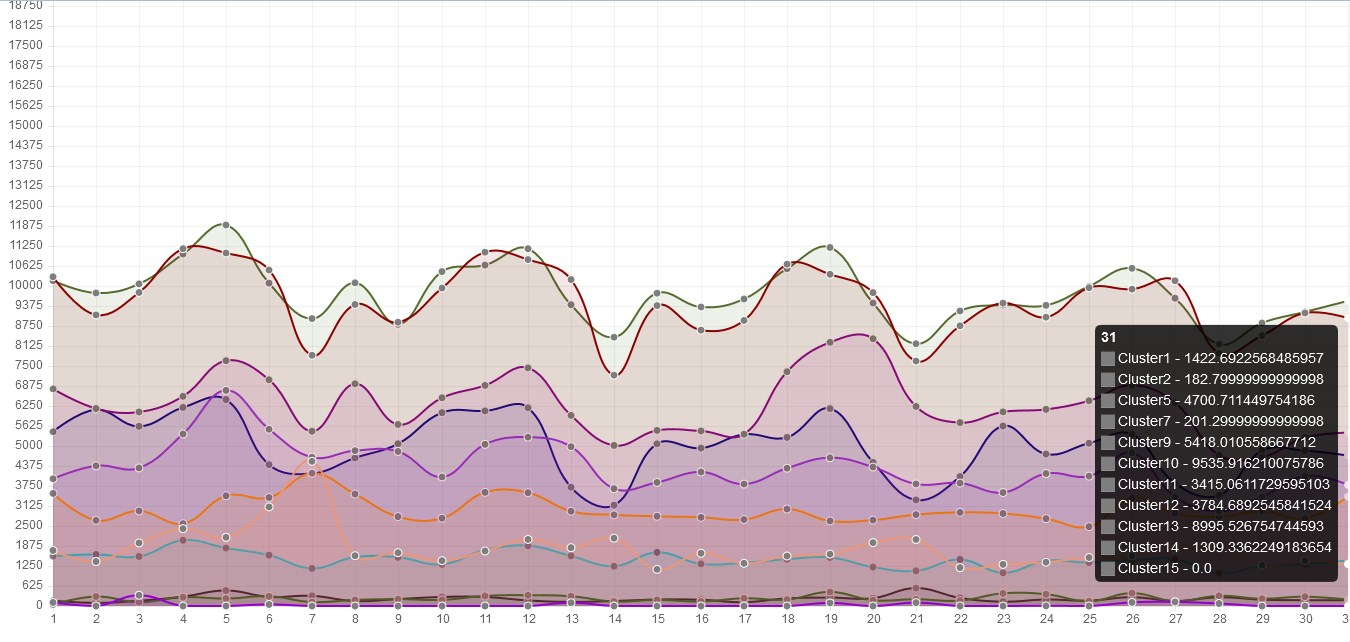
\includegraphics[width=0.8\linewidth]{Line/Line_All_Cost.jpg}
	\caption{Data total cost setiap cluster}
\end{figure}

\begin{figure}[H]
	\centering
	\includegraphics[width=0.8\linewidth]{Line_All_Probability.jpg}
	\caption{Data total cost setelah dikonversi menjadi probabilitas}
\end{figure}

Dari hasil tersebut dilakukan plotting data dengan perkembangan profit  untuk setiap bulannya, hasil visualisasi tersebut adalah sebagai berikut:

\begin{figure}[H]
	\centering
	\begin{minipage}{.5\textwidth}
		\centering
		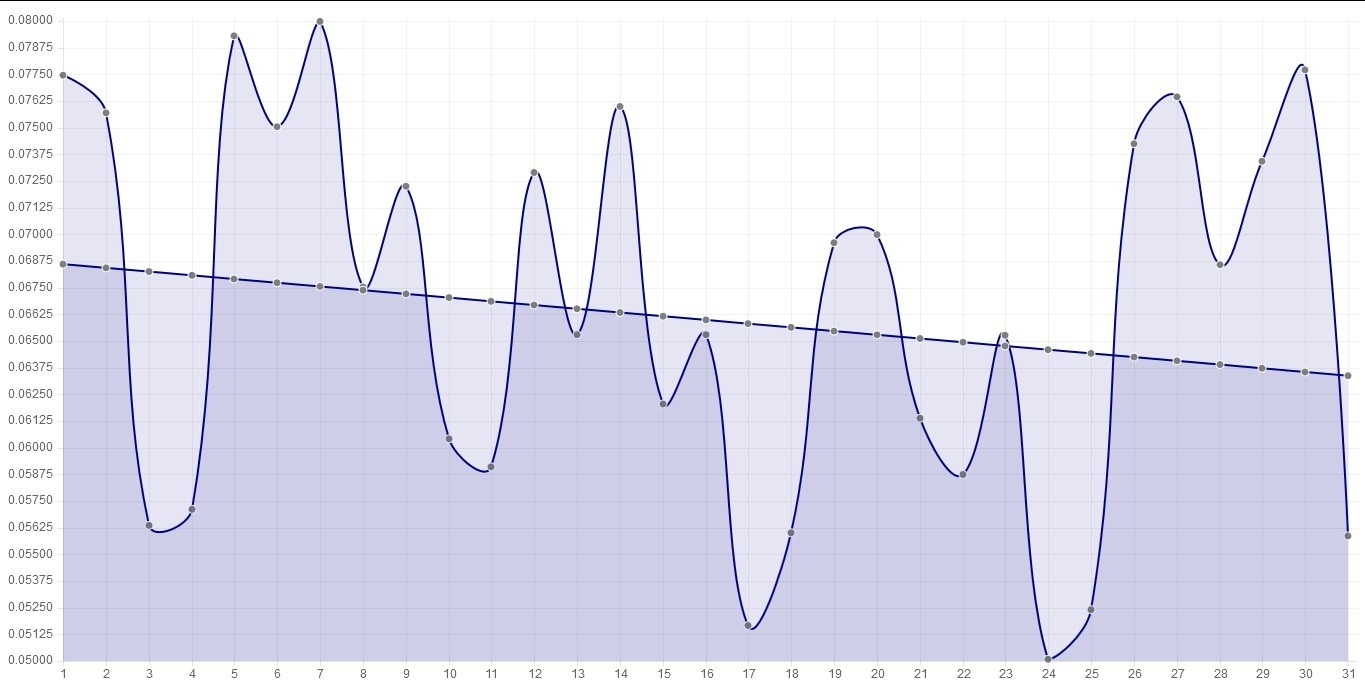
\includegraphics[width=.9\linewidth]{Line/Line_Anomaly_02.jpg}
		\captionof{figure}{Visualisasi Bulan Kedua$\\KL Divergence = 0.015632698168624958\\$}
	\end{minipage}%
	\begin{minipage}{.5\textwidth}
		\centering
		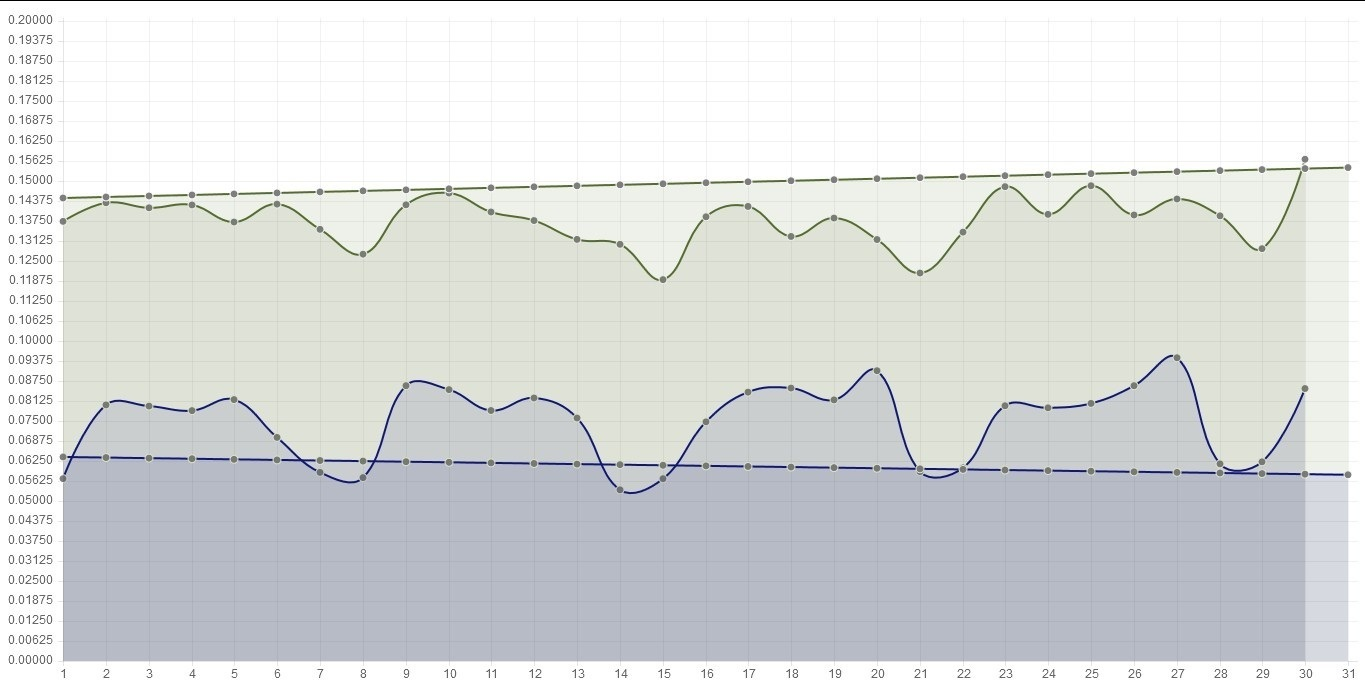
\includegraphics[width=.9\linewidth]{Line/Line_Anomaly_03.jpg}
		\captionof{figure}{Visualisasi Bulan Ketiga$\\KL Divergence Top = 0.044998303321150374\\KL Divergence Bot = 0.026714006810494257$}
	\end{minipage}%
\end{figure}

\begin{figure}[H]
	\centering
	\begin{minipage}{.5\textwidth}
		\centering
		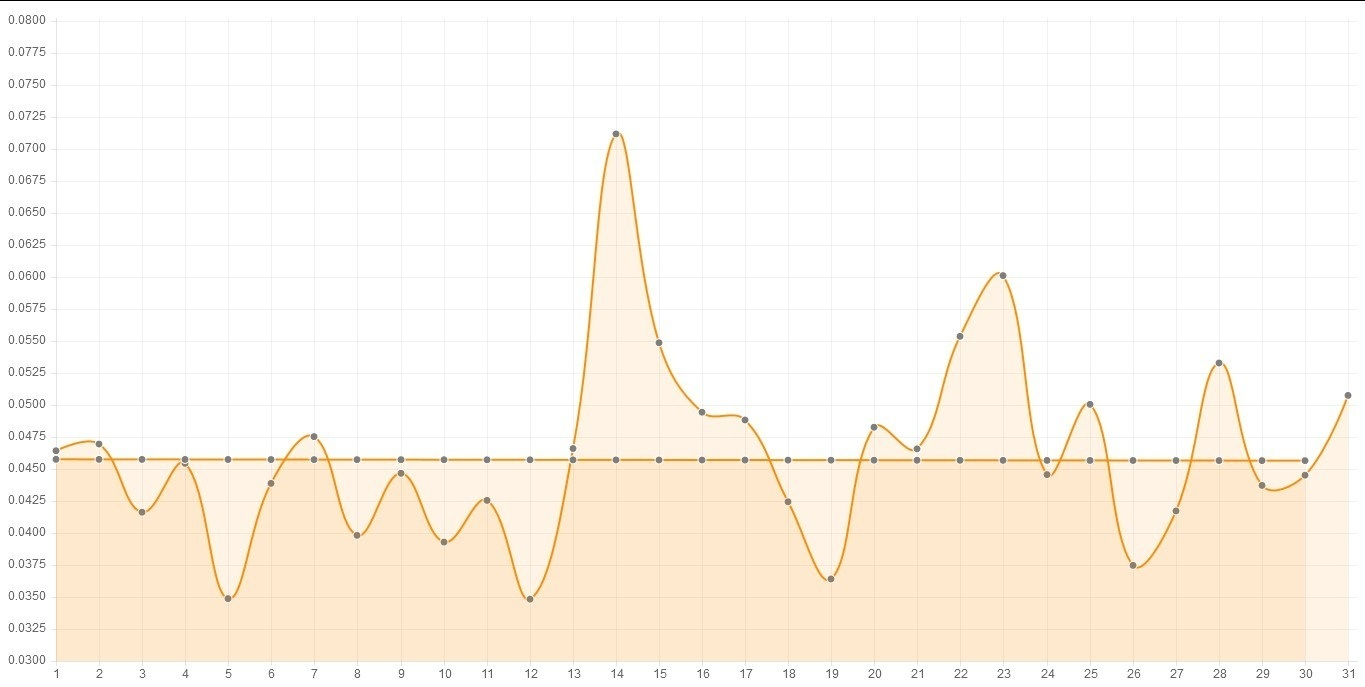
\includegraphics[width=.9\linewidth]{Line/Line_Anomaly_04.jpg}
		\captionof{figure}{Visualisasi Bulan Keempat$\\KL Divergence = 0.03152148657242697$}
	\end{minipage}%
	\begin{minipage}{.5\textwidth}
		\centering
		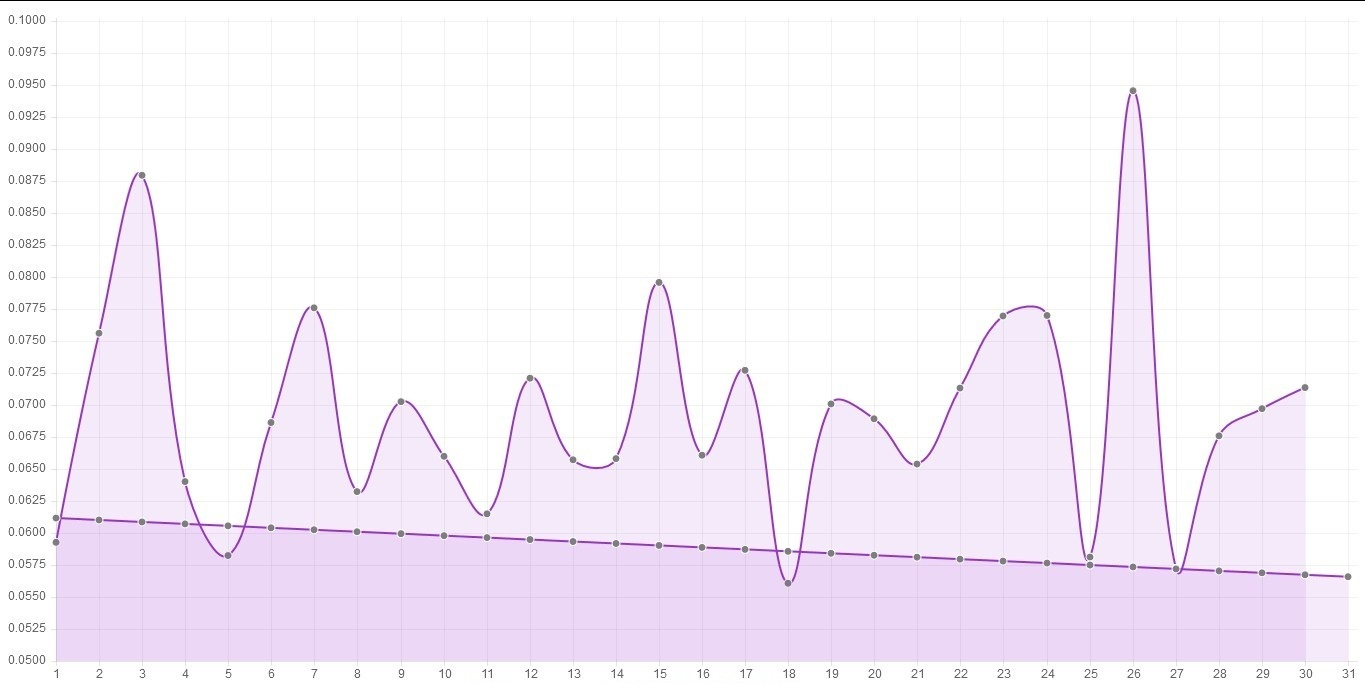
\includegraphics[width=.9\linewidth]{Line/Line_Anomaly_05.jpg}
		\captionof{figure}{Visualisasi Bulan Kelima$\\KL Divergence = 0.0472788377243259$}
	\end{minipage}%
\end{figure}

\begin{figure}[H]
	\centering
	\begin{minipage}{.5\textwidth}
		\centering
		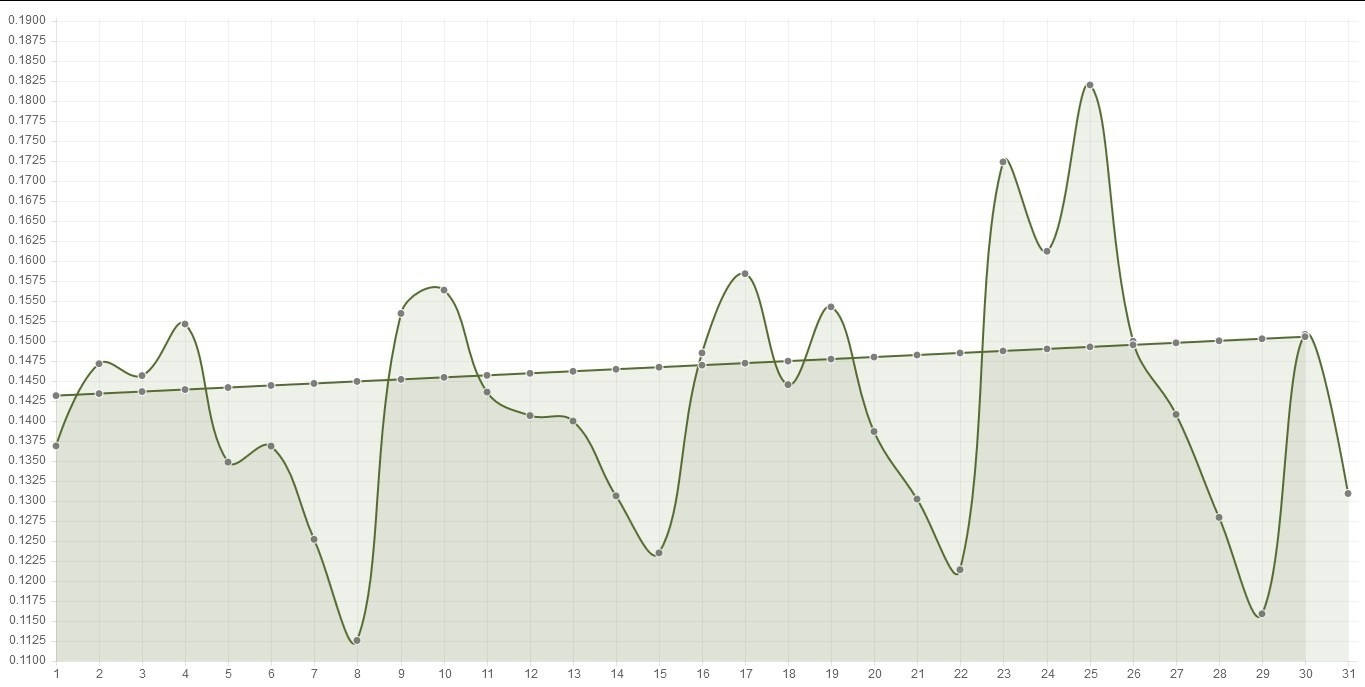
\includegraphics[width=.9\linewidth]{Line/Line_Anomaly_06.jpg}
		\captionof{figure}{Visualisasi Bulan Keenam$\\KL Divergence = 0.036093264517592136$}
	\end{minipage}%
	\begin{minipage}{.5\textwidth}
		\centering
		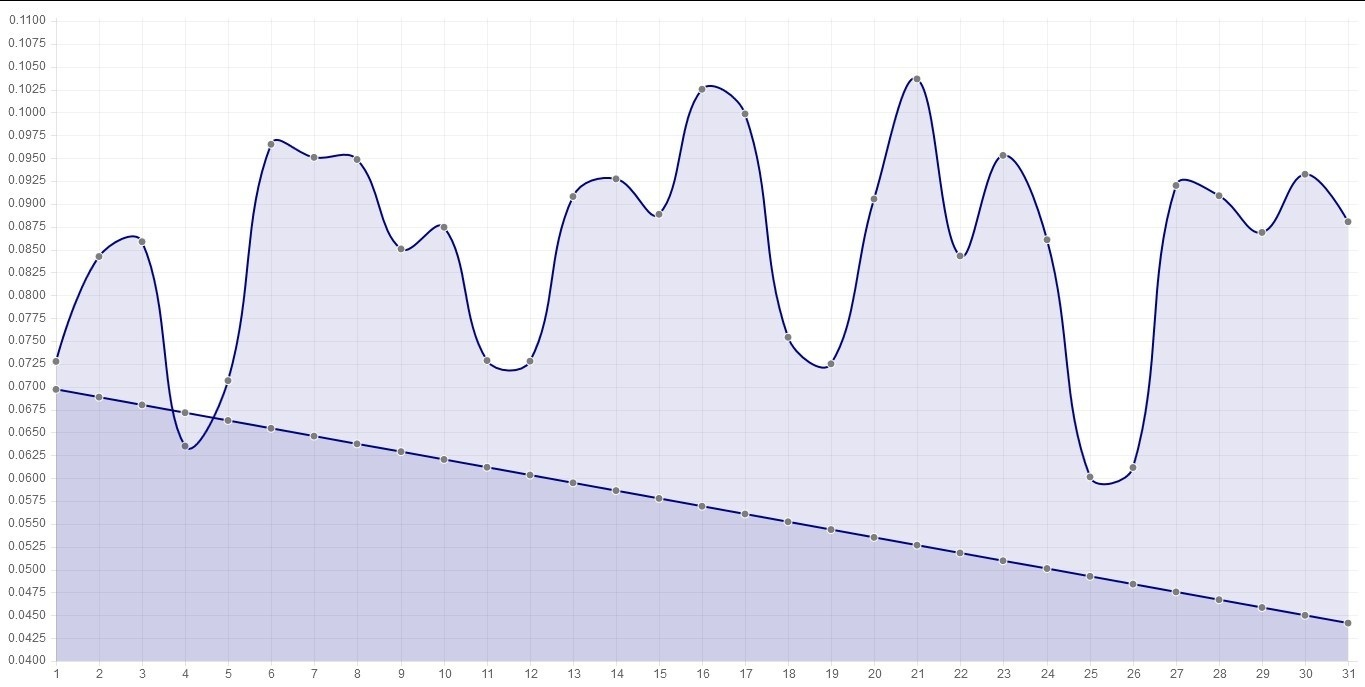
\includegraphics[width=.9\linewidth]{Line/Line_Anomaly_07.jpg}
		\captionof{figure}{Visualisasi Bulan Ketujuh$\\KL Divergence = 0.07018660930043484$}
	\end{minipage}%
\end{figure}

\begin{figure}[H]
	\centering
	\begin{minipage}{.5\textwidth}
		\centering
		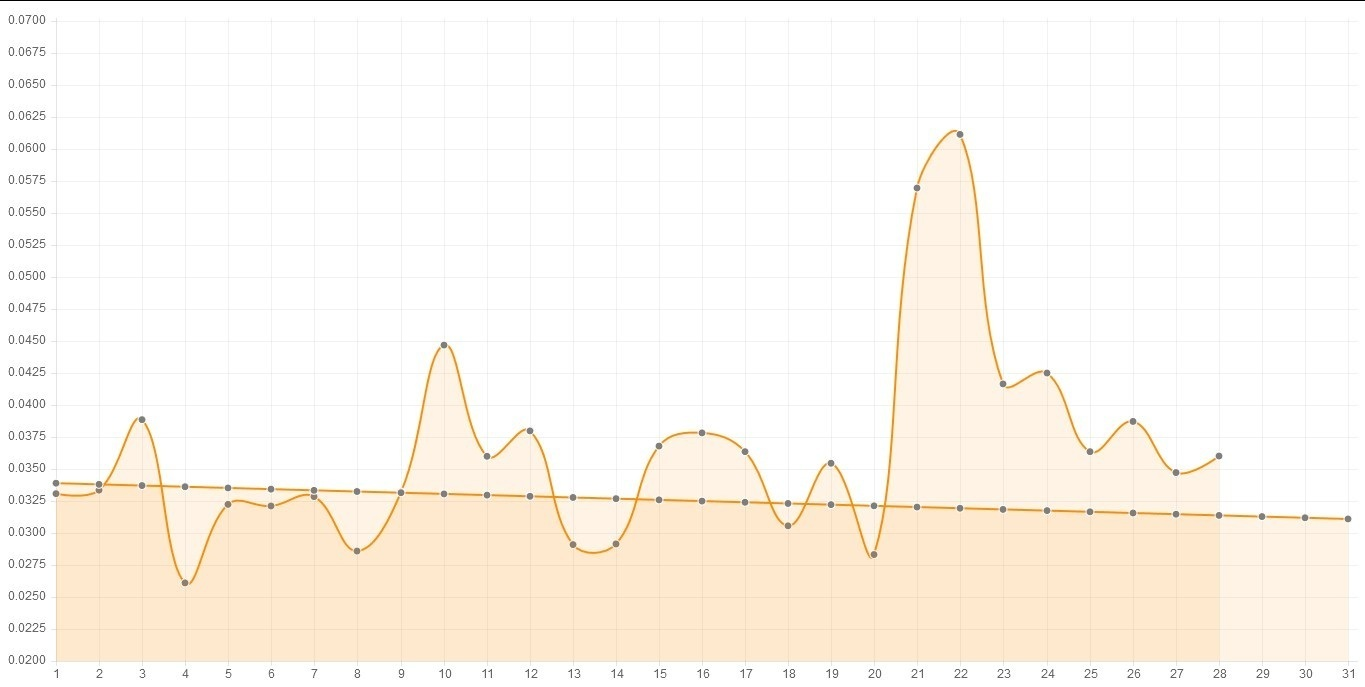
\includegraphics[width=.9\linewidth]{Line/Line_Anomaly_08.jpg}
		\captionof{figure}{Visualisasi Bulan Kedelapan$\\KL Divergence = 0.039705311189136054$}
	\end{minipage}%
	\begin{minipage}{.5\textwidth}
		\centering
		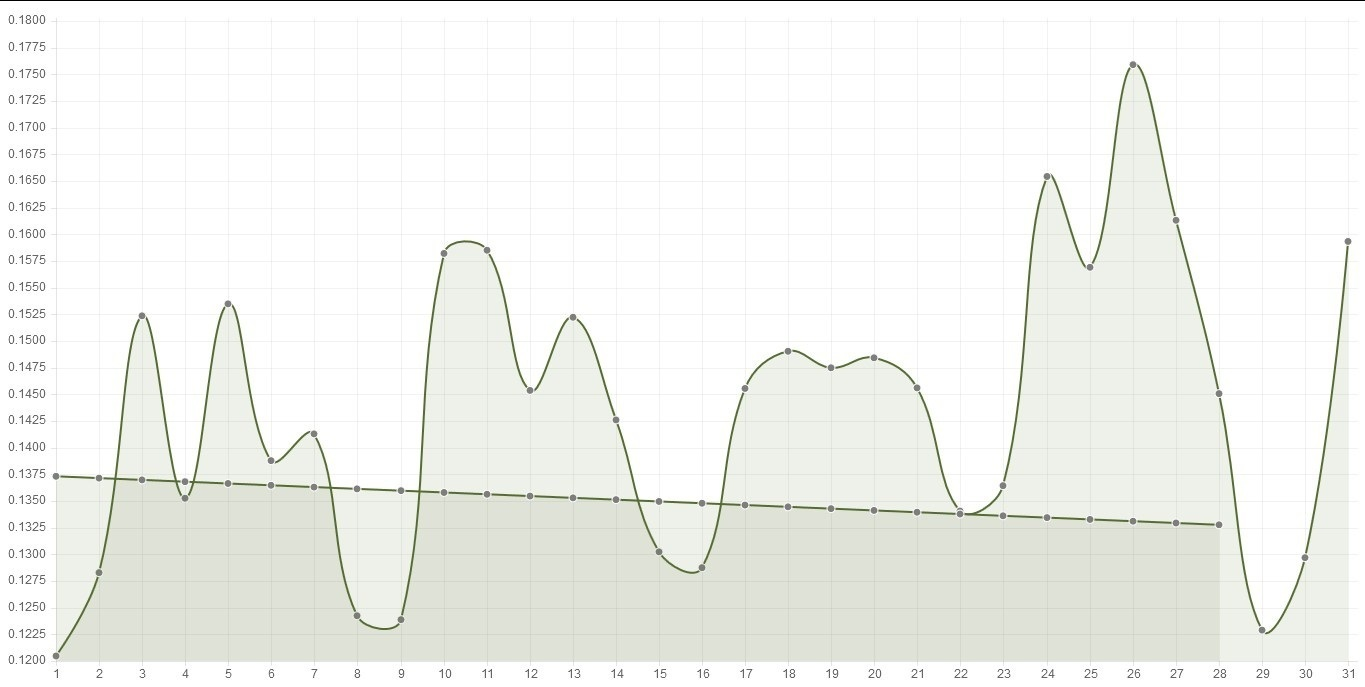
\includegraphics[width=.9\linewidth]{Line/Line_Anomaly_09.jpg}
		\captionof{figure}{Visualisasi Bulan Ketiga$\\KL Divergence = 0.04904454504562369$}
	\end{minipage}%
\end{figure}

\begin{figure}[H]
	\centering
	\begin{minipage}{.5\textwidth}
		\centering
		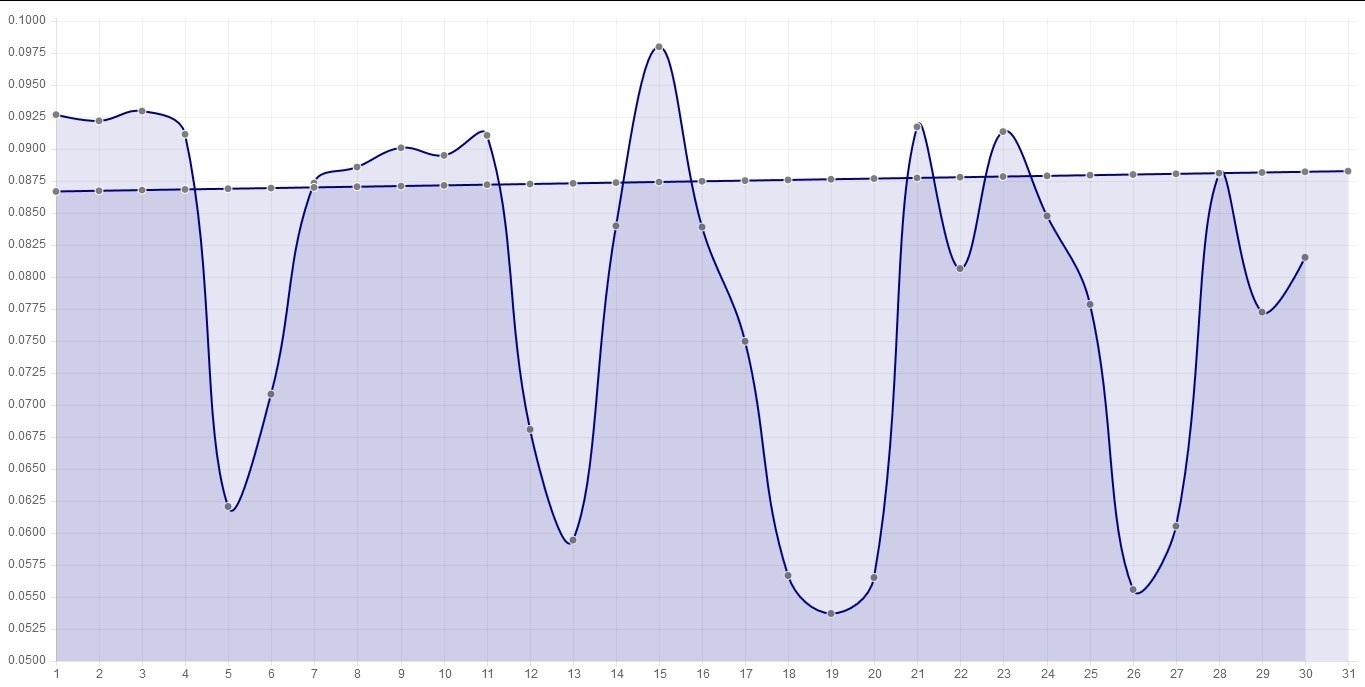
\includegraphics[width=.9\linewidth]{Line/Line_Anomaly_10.jpg}
		\captionof{figure}{Visualisasi Bulan Kesepuluh$\\KL Divergence = 0.026295761592674213$}
	\end{minipage}%
	\begin{minipage}{.5\textwidth}
		\centering
		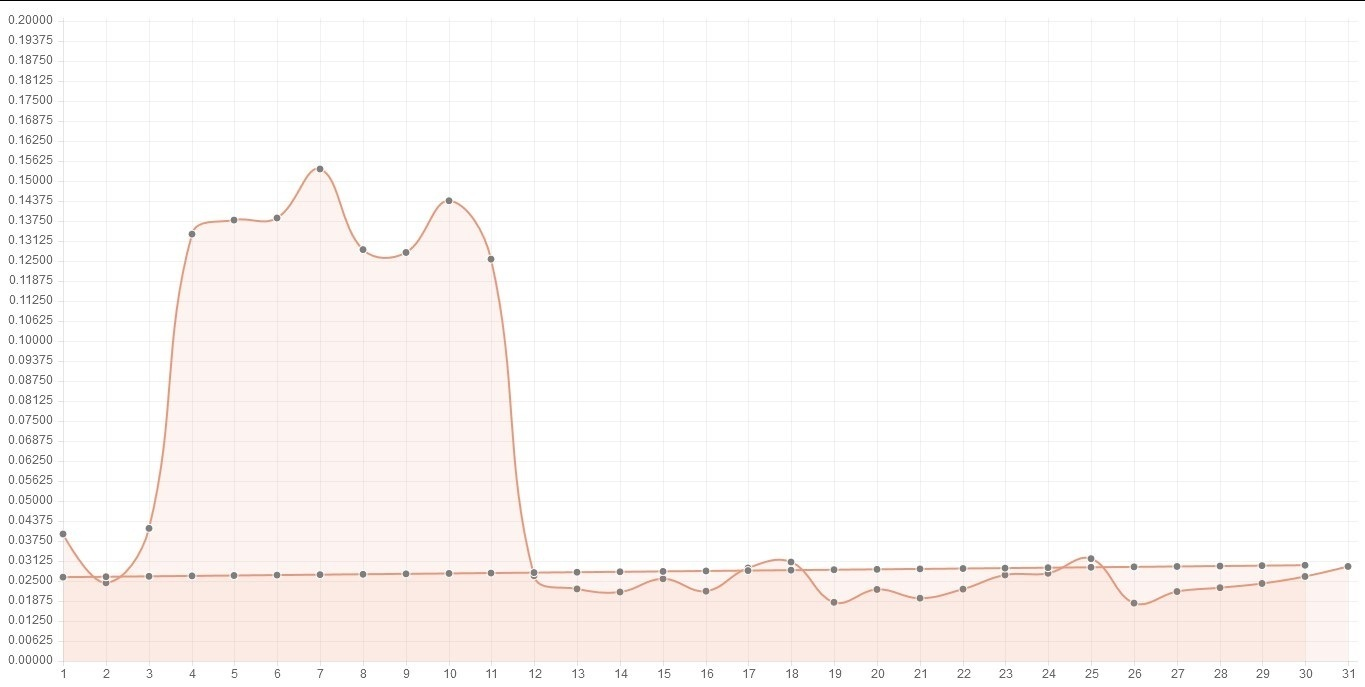
\includegraphics[width=.9\linewidth]{Line/Line_Anomaly_11.jpg}
		\captionof{figure}{Visualisasi Bulan Kesebelas$\\KL Divergence = 0.26752695868379334$}
	\end{minipage}%
\end{figure}

\begin{figure}[H]
	\centering
	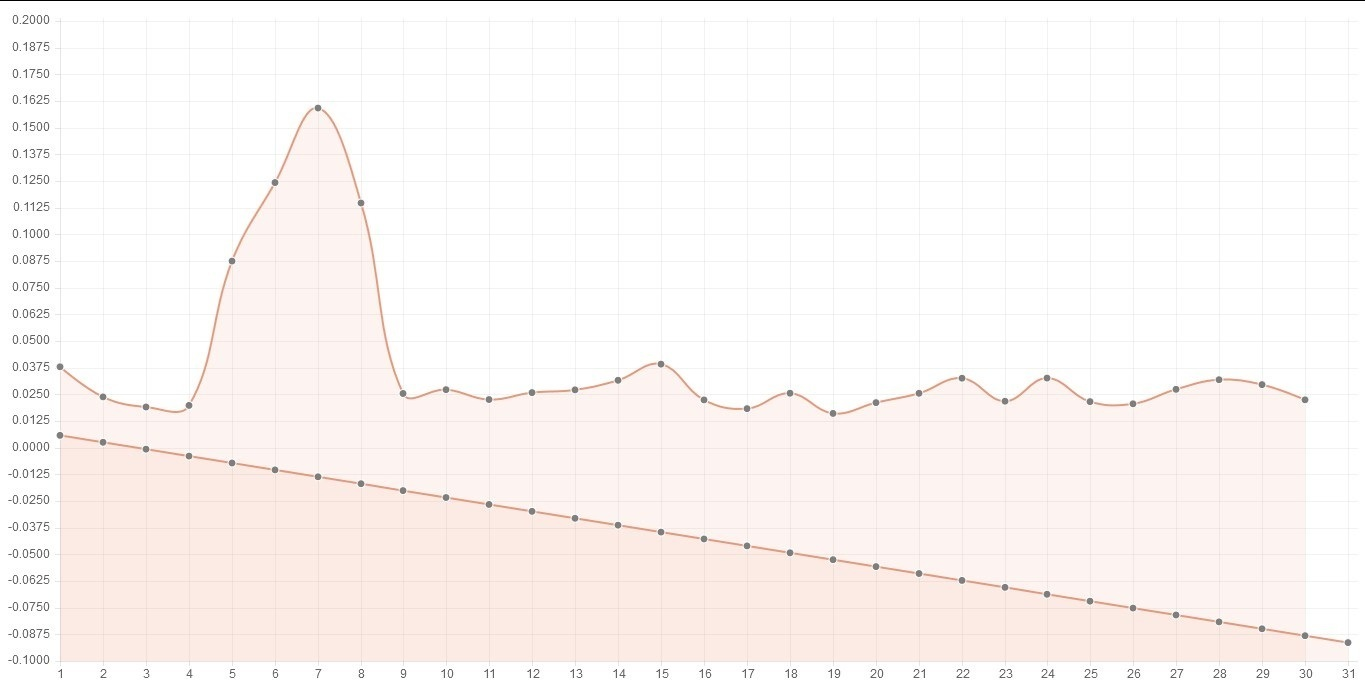
\includegraphics[width=.45\linewidth]{Line/Line_Anomaly_12.jpg}
	\caption{Visualisasi Bulan Keduabelas\\$KL Divergence = 0.07129923008134906$}
\end{figure}

Dari hasil keseluruhan tersebut fenomena anomali dengan  perbedaan keuntungan paling tinggi (nilai divergen paling tinggi) terdapat pada bulan 10, yaitu cluster yang terpusat pada daerah Matosinhos. Pada tanggal 4 sampai 11 terdapat kenaikan profit yang sangat signifikan dan kembali pada distribusi sebelumnya setelah interval waktu tersebut. Figure p ke q merupakan  plotting frekuensi pemesanan taxi pada peta berdasarkan lokasi gps pada data. daerah Matosinhos mengalami kenaikan frekuensi pemesanan taxi dalam jumlah besar.

\begin{figure}[H]
	\centering
	\begin{minipage}{.4\textwidth}
		\centering
		\includegraphics[width=\linewidth]{Month_09_CropMarked.jpg}
		\captionof{figure}{Plot Frekuensi Penggunaan Taksi Bulan Kesembilan}
	\end{minipage}%
	\hspace{.1\textwidth}
	\begin{minipage}{.4\textwidth}
		\centering
		\includegraphics[width=\linewidth]{Month_10_CropMarked.jpg}
		\captionof{figure}{Plot Frekuensi Penggunaan Taksi Bulan Kesepuluh}
	\end{minipage}%
\end{figure}

\begin{figure}[H]
	\centering
	\begin{minipage}{.4\textwidth}
		\centering
		\includegraphics[width=\linewidth]{Month_11_CropMarked.jpg}
		\captionof{figure}{Plot Frekuensi Penggunaan Taksi Bulan Kesebelas}
	\end{minipage}%
	\hspace{.1\textwidth}
	\begin{minipage}{.4\textwidth}
		\centering
		\includegraphics[width=\linewidth]{Month_12_CropMarked.jpg}
		\captionof{figure}{Plot Frekuensi Penggunaan Taksi Bulan Keduabelas}
	\end{minipage}%
\end{figure}

\section{Kesimpulan}

Dengan menggunakan k-means clustering dengan pemilihan jumlah cluster yang tepat, daerah-daerah yang berdekatan dapat dikelompokkan menjadi kelompok-kelompok yang terpisah dan modular. Centroid setiap cluster juga memudahkan penentuan representasi cluster-cluster tersebut.

Implementasi model regresi yang tepat pada suatu data dapat mempengaruhi hasil estimasi data dan mempengaruhi seberapa cocok regresi tersebut terhadap data asli, seperti pada kasus ini, prediksi menggunakan regresi linier pada data monoton (isotonic regression) memberikan hasil yang lebih representatif dibandingkan data yang tidak monoton.

Penghitungan divergensi profit menggunakan KL-Divergence mampu mendeteksi perkembangan keuntungan penggunaan jasa taxi secara cepat dan akurat.

\end{document}